\documentclass[11pt]{article}

\usepackage{amsmath}
\usepackage[margin=0.68in]{geometry}
\usepackage{booktabs}
\usepackage{enumitem}
\usepackage{fancyhdr}
\usepackage{graphicx}
\usepackage[table]{xcolor}
\usepackage[hidelinks]{hyperref}
\usepackage{listings}
\usepackage{microtype}
\usepackage{tabularx}
\usepackage{titlesec}
\graphicspath{{docs/lessons/assets/}{../assets/}}

\definecolor{Ink}{gray}{0}
\definecolor{CodeGray}{gray}{0.96}
\hypersetup{
  hidelinks,
  pdftitle={ADK Lesson 034: Magnetic Observations},
  pdfauthor={Kevin Shanahan},
  pdfsubject={Qualified magnetic observations, dwell, hysteresis, explicit-time evidence, and specimen gates},
  pdflang={en-US}
}
\pagestyle{fancy}
\fancyhf{}
\lhead{\textsc{ADK Lesson 034}}
\rhead{Magnetic Observations}
\cfoot{\thepage}
\setlength{\headheight}{14pt}
\setlength{\parindent}{0pt}
\setlength{\parskip}{5pt}
\setlist{nosep,leftmargin=1.45em}
\titleformat{\section}{\Large\bfseries\color{Ink}}{\thesection}{0.5em}{}
\lstdefinestyle{adkcpp}{
  language=C++,
  backgroundcolor=\color{CodeGray},
  basicstyle=\ttfamily\small,
  keywordstyle=\color{Ink}\bfseries,
  commentstyle=\color{Ink},
  columns=fullflexible,
  keepspaces=true,
  showstringspaces=false,
  frame=single,
  rulecolor=\color{Ink},
  breaklines=true,
  tabsize=4
}
\newcommand{\lessonbox}[1]{%
  \begin{center}\fcolorbox{Ink}{white}{\parbox{0.92\linewidth}{#1}}\end{center}}

\begin{document}

\begin{center}
  {\Huge\bfseries Magnetic Observations}\\[4pt]
  {\Large Preserve raw evidence before interpreting a boundary}\\[8pt]
  \textit{One sample, one timestamp, one stable snapshot}
\end{center}

\begin{tabularx}{\linewidth}{@{}>{\bfseries}l X >{\bfseries}l X@{}}
Lesson & 034 --- component & Time & 120--180 minutes\\
Prerequisites & Lessons 002, 007, and 008 & Board & Arduino Mega 2560\\
Evidence & TP-H, TP-R, three LED witnesses & Status & host verified; bench open\\
Energy class & E0 host; provisional E1 fixture after specimen qualification\\
\end{tabularx}

\lessonbox{\textbf{Specimen gate.} The authorized inventory lists ``Linear
Hall'' and ``Magnetic Spring'' families. It does not establish output type,
pin order, voltage, pull-up rail, polarity, active level, transfer curve, or a
safe magnetic stimulus. Keep both specimens unpowered and quarantined until
their exact markings and primary electrical evidence resolve every role.}

\section{Mission and learning outcomes}

The lesson separates three layers:
\[
\text{raw sample}\rightarrow\text{qualified range and dwell}
\rightarrow\text{stable magnetic observation}.
\]

By the end, you can:
\begin{itemize}
  \item preserve an ADC count or contact level beside its interpretation;
  \item distinguish out-of-range evidence from an invented fault diagnosis;
  \item apply hysteresis and continuous dwell without blocking;
  \item explain why a digital contact has no inferred magnetic polarity;
  \item reject backward time while accepting natural timestamp rollover;
  \item prove resource acquisition separately from shutdown pin state.
\end{itemize}

\section{Inspect before any powered circuit}

\begin{center}
% ADK visual: pencil
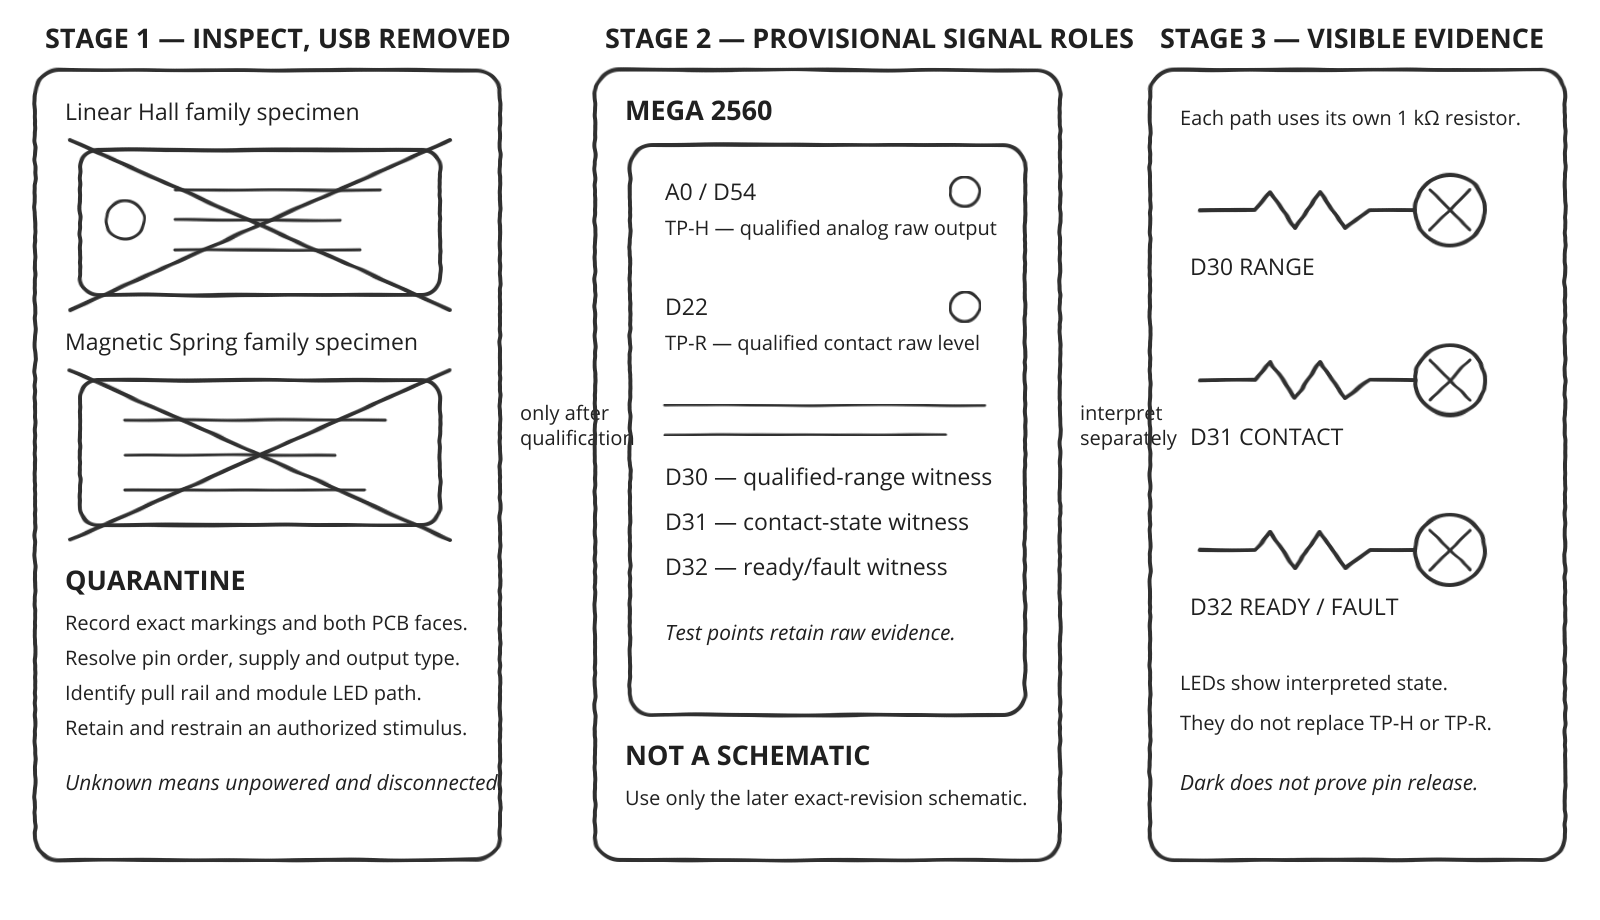
\includegraphics[width=0.96\linewidth]{034-magnetic-observation-pencil.png}

\small\textit{Alternative text: pencil inspection plate showing two
unidentified magnetic-family specimens crossed out and quarantined until
qualified, then a Mega observation stage with TP-H and TP-R leading to three
resistor-limited evidence LEDs.}
\end{center}

The drawing is an orientation and decision path, not an electrical schematic.
No electrically authoritative schematic is possible until the exact retained
specimens are identified. With USB absent, record both PCB faces, markings,
connector labels, continuity-safe ground evidence, supply rating, output
topology, pull rail, module LED path, and maximum current. A cracked glass
capsule, ambiguous mercury-like part, unresolved pinout, or loose magnetic
stimulus stops the physical route.

\begin{tabularx}{\linewidth}{@{}l l X@{}}
\toprule
Evidence point & Provisional Mega pin & Meaning after qualification\\
\midrule
TP-H & A0 / D54 & retained linear-family raw ADC output\\
TP-R & D22 & retained contact-family raw digital output\\
range LED & D30 through 1 k\(\Omega\) & TP-H lies inside configured range\\
contact LED & D31 through 1 k\(\Omega\) & contact observation is active\\
ready/fault LED & D32 through 1 k\(\Omega\) & acquisition and current health\\
\bottomrule
\end{tabularx}

\section{Linear observation contract}

\texttt{LinearHall} owns one \texttt{AnalogInput}. Its configured ordering is:
\[
q_{\min}\le n_a<n_r<p_r<p_a\le q_{\max}\le1023.
\]
Here \(n_a,n_r\) are negative activate/release thresholds and \(p_r,p_a\)
are positive release/activate thresholds. The separated bands prevent one
noisy count from repeatedly changing the stable interpretation.

A candidate polarity must remain continuously present for \texttt{dwell}.
Travel directly from Negative evidence to Positive evidence first qualifies a
Neutral interval and emits deactivation; only a later distinct dwell can emit
the new activation. Optional reversal swaps the reported Negative and Positive
labels after interpretation. It does not alter the retained raw count.

\begin{tabularx}{\linewidth}{@{}l X@{}}
\toprule
Snapshot field & Meaning\\
\midrule
\texttt{raw}, \texttt{observedAt} & exact retained ADC sample and caller time\\
\texttt{polarity} & stable Negative, Neutral, or Positive interpretation\\
\texttt{activationEvent}, \texttt{deactivationEvent} & transition from the latest update only\\
\texttt{stableFor} & modular duration of the current stable interpretation\\
\texttt{quality} & Valid, below range, above range, or unqualified\\
\texttt{status} & lifecycle or time-contract result\\
\bottomrule
\end{tabularx}

Below- or above-range evidence clears a pending candidate. It does not claim
open circuit, short circuit, missing magnet, saturation, or a damaged module.
Those hypotheses require independent electrical evidence.

\begin{center}
% ADK visual: pencil
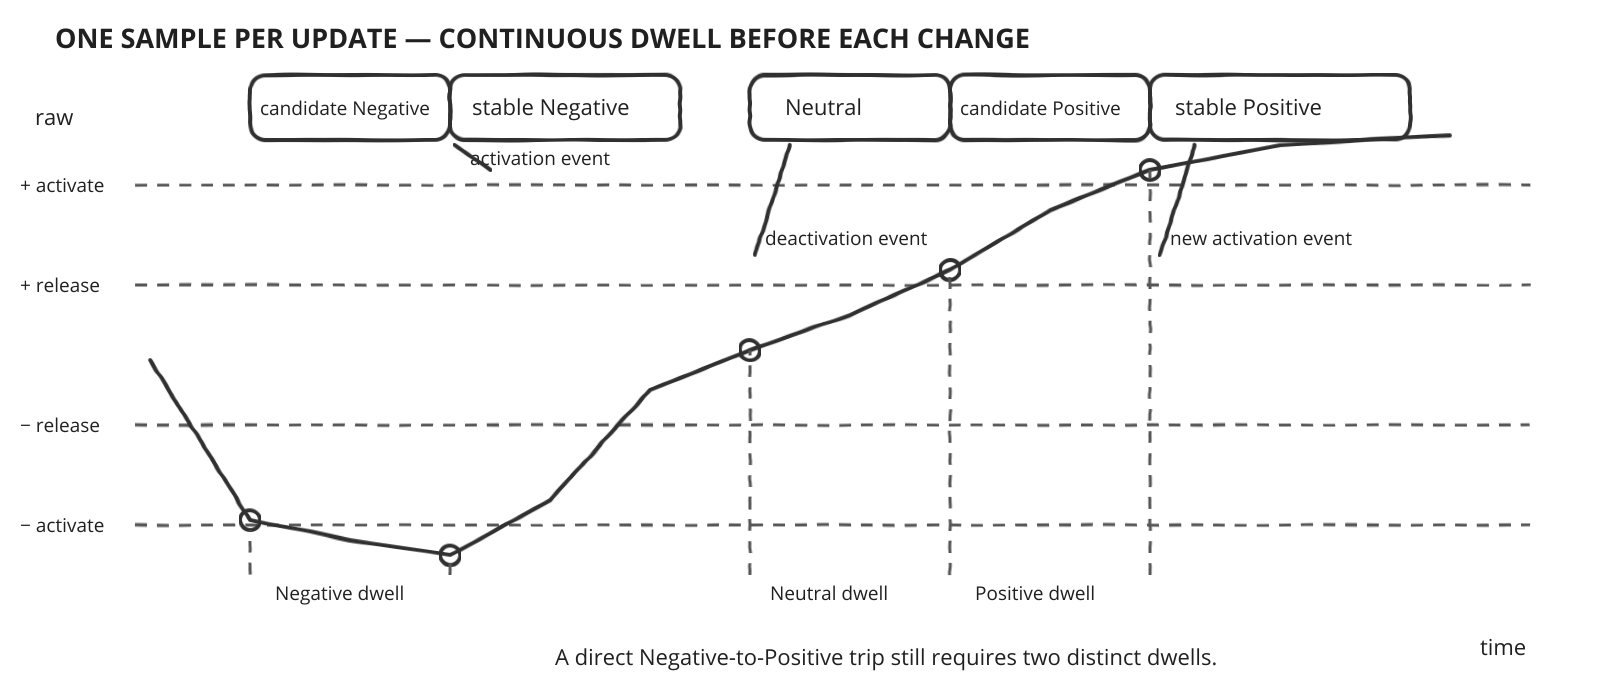
\includegraphics[width=0.96\linewidth]{034-magnetic-transition-pencil.png}

\small\textit{Alternative text: pencil timing plate showing raw samples
qualifying Negative after continuous dwell, returning through a separately
qualified Neutral dwell with deactivation, then qualifying Positive in a new
dwell before activation.}
\end{center}

Use the plate as three dependent visible stages: first retain the raw trace,
then mark a candidate only while every sample remains in its band, and only
then compare the stable observation and event witness. A band exit erases the
unfinished candidate; it does not erase the retained sample.

\section{Contact observation contract}

\texttt{MagneticContact} owns one \texttt{DigitalInput} with explicit pull,
closed level, and dwell. Its canonical raw value is zero for Low and one for
High. Its polarity is always \texttt{Unspecified}: one contact cannot establish
field direction. Constant open or closed evidence likewise cannot distinguish
a steady stimulus from a stuck, shorted, or disconnected circuit.

Both components construct inertly, validate before claiming, sample exactly
once per explicit-time update, and retain a stable snapshot until the next
update. Failed initialization leaks no claim. Repeated initialization and
shutdown are idempotent; destruction releases the owned input.

\section{Time and deterministic replay}

Unsigned modular elapsed time strictly below \(2^{31}\) milliseconds advances.
Natural 32-bit rollover is therefore valid. An exact half-range or larger
apparent jump is rejected as \texttt{InvalidArgument} without sampling or
changing transition state. A replay using the same configuration, raw samples,
and timestamps produces the same snapshots and pin-operation trace.

\section{Narrative Mega example}

\begin{lstlisting}[style=adkcpp]
void loop ()
{
    const adk::TimePoint now (millis ());

    observeMagneticInputs (now);

    if (!decideEvidence () || !actuateEvidence ())
    {
        stopSafely ();
    }
}
\end{lstlisting}

The canonical sketch acquires the two observers and three \texttt{MonoLed}
witnesses, configures a bounded run, starts with ready evidence, then preserves
observe--decide--actuate order. It stops independently after 120 seconds.
Serial is unnecessary.

\section{Predict, observe, interpret}

\begin{enumerate}
  \item Before connecting anything, predict which marking or source will
        establish each specimen role. If any role remains inferred, stop.
  \item With a qualified, unpowered fixture, predict TP-H and TP-R idle values
        and each LED's current bound. Check every 1 k\(\Omega\) resistor.
  \item Apply USB power. Observe the ready witness separately from the two raw
        test points. Interpret ready only as resource-acquisition evidence.
  \item Move only the separately authorized retained stimulus through the
        documented fixture. Predict raw range, dwell, and event order before
        observing TP-H and the range witness.
  \item Exercise the qualified contact without flexing a glass capsule.
        Compare raw level, stable state, and contact witness through bounce.
  \item Invoke shutdown. Predict dark LEDs and released input pins. Measure the
        named safe state separately; darkness alone does not prove release.
\end{enumerate}

\section{Diagnosis and stop conditions}

\begin{tabularx}{\linewidth}{@{}X X@{}}
\toprule
Observation & Stop, inspect, and interpret\\
\midrule
unknown marking or pin order & remain unpowered; obtain exact primary evidence\\
TP-H outside the qualified rail & remove USB; inspect supply and output topology\\
range witness chatters & compare raw counts, thresholds, dwell, and ground\\
contact never changes & retain raw level; do not guess stuck versus absent stimulus\\
event skips Neutral & inspect the trace and separate the two dwell intervals\\
hot part, odor, reset, or unstable rail & remove USB immediately\\
loose stimulus or cracked capsule & quarantine the fixture; do not continue\\
\bottomrule
\end{tabularx}

\section{Exercises}

\begin{enumerate}
  \item Draw the five ordered thresholds and mark the two hysteresis bands.
  \item Explain why reversal changes polarity labels but not raw evidence.
  \item Give a rollover trace that advances five milliseconds across zero.
  \item Show the reverse rollback order after the second observer cannot claim
        its pin.
  \item List three hypotheses for a constant contact and the additional
        evidence needed to distinguish them.
\end{enumerate}

\lessonbox{\textbf{Stop rule.} Remove USB for heat, odor, reset or rail
instability, current-limit trip, out-of-rail output, unexpected movement,
specimen/source disagreement, loose stimulus, cracked capsule, or current
above a pin, port, package, rail, or aggregate budget. Change wiring only
while unpowered. Never create a live short.}

\section{Software evidence and reference trail}

Repository automation verifies threshold boundaries, dwell, hysteresis,
reversal, chatter, rollover, backward time, invalid configuration, busy pins,
rollback, reuse, ownership traits, Mega compilation, size, and publication.
These are host claims, not physical observations.

The searchable HTML lesson is the primary accessible route. Consult the
magnetic-observation interface, focused tests, canonical sketch, Lessons
034--036 design record, repository policies, authorized family manifest, and
exact-specimen primary sources.
This PDF remains untagged and makes no PDF/UA claim.

\end{document}
